\section{Organisation du projet}
    \subsection{Planning prévisionnel}

        \begin{figure}[h]
            \centering
            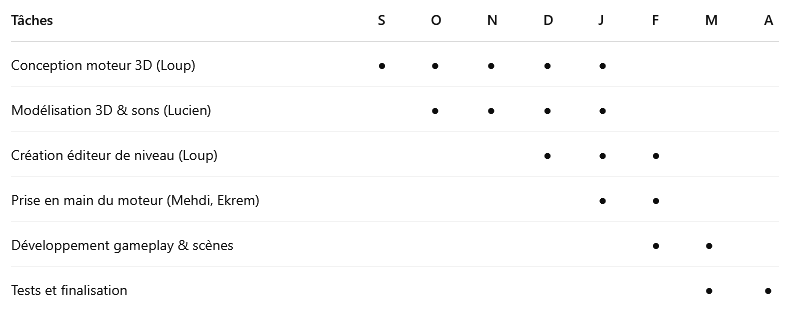
\includegraphics[width=0.6\textwidth]{images/gantt_previsionnel.png}
            \caption{Gantt prévisionnel}
            \label{fig:gantt_previsionnel}
        \end{figure}
        Dès les prémices du projet Chapper's Fallout, une planification claire et structurée a été établie, plusieurs mois avant le lancement effectif du développement. 
        Cette anticipation visait à garantir une répartition cohérente des rôles, adaptée aux compétences et à l'expérience de chaque membre de l'équipe.
        \\ \\
        Loup, le membre le plus expérimenté en développement de jeux vidéo, a été naturellement désigné responsable de la conception et de la mise en place du moteur 3D. 
        Son rôle central consistait à fournir les fondations techniques du jeu : moteur de rendu, système d’entrée/sortie, structure de données, ainsi qu’un éditeur de 
        niveau pour faciliter le travail des autres membres.
        \\ \\
        Lucien, de son côté, s’est vu confier la création des ressources graphiques et sonores : modélisation 3D de la carte et des objets, textures, musiques et effets 
        sonores, apportant une identité visuelle et sonore au jeu.
        \\ \\
        Mehdi et Ekrem, moins expérimentés en développement 3D au démarrage du projet, devaient capitaliser sur les outils fournis par Loup ( notamment l’éditeur de niveau  
        ) pour implémenter des fonctionnalités concrètes du jeu. Leur mission initiale était donc orientée vers des tâches techniques réalisables et progressives, comme la 
        gestion d’objets interactifs, des scènes ou encore l’intégration de mini-jeux.
        \\ \\
        Ce planning prévisionnel reposait ainsi sur une forte complémentarité des compétences : Loup assurait la direction technique et le développement du socle du jeu, 
        pendant que les autres membres construisaient progressivement les éléments du gameplay, tout en se formant à mesure de l’avancement du projet.
        \\ \\
        Afin d’assurer le bon déroulement du projet, une stratégie spécifique a été mise en place dès le départ. Conscients que la réussite globale dépendait en grande 
        partie de la création du moteur 3D, nous avons décidé que Loup commencerait son développement bien en amont, plusieurs mois avant le lancement officiel des séances 
        de projet. Cette avance lui permettait de poser des bases techniques solides sur lesquelles le reste de l’équipe pourrait s’appuyer. Parallèlement, Mehdi et Ekrem 
        avaient pour objectif de se familiariser rapidement avec ce moteur, afin de pouvoir intervenir efficacement sur le développement des différentes fonctionnalités du 
        jeu. De son côté, Lucien devait produire une première version fonctionnelle du modèle 3D assez tôt, ce qui permettrait de tester les interactions en jeu et de 
        débuter le codage des mécaniques. La suite du travail de modélisation visuelle pouvait ensuite se dérouler de manière plus progressive, en respectant les délais 
        impartis.


    \subsection{Répartition des tâches}
        Tout au long du développement de Chapper's Fallout, notre groupe a su faire preuve d’une forte capacité d’adaptation face aux imprévus et aux défis techniques rencontrés. 
        Si les rôles de Loup et Lucien sont restés globalement stables, Loup étant responsable du moteur 3D et Lucien de la modélisation 3D et des ressources sonores, les 
        tâches initialement confiées à Ekrem et Mehdi ont quant à elles évolué au fil du projet, en réponse aux réalités du terrain.
        \\ \\
        À l’origine, Mehdi et Ekrem devaient s’occuper du développement des \\fonctionnalités du jeu, en exploitant le moteur mis en place par Loup. Cependant, cette mission 
        s’est avérée ambitieuse compte tenu de leur niveau initial en programmation 3D. Très tôt dans le projet, une remise en question collective a permis de recentrer 
        leurs objectifs vers des tâches plus ciblées et adaptées : la création de mini-jeux en 2D avec SDL, destinés à enrichir l’expérience de jeu tout en s’inscrivant 
        dans un cadre technique plus accessible.
        \\ \\
        Par ailleurs, l’équipe a su faire face à un autre ajustement majeur concernant la gestion des collisions. Initialement, cette tâche devait être assurée par Lucien. 
        Cependant, la charge de travail en modélisation 3D s’est révélée plus importante que prévu, notamment pour finaliser les nombreux éléments visuels du jeu dans les 
        temps. Pour permettre à Lucien de se concentrer pleinement sur cette mission essentielle, la responsabilité des collisions a été transférée à Mehdi. Ce dernier a 
        alors assumé avec efficacité cette tâche minutieuse et critique, qui nécessitait une intervention manuelle dans les scènes 3D. 
        \\ \\
        Ces ajustements successifs témoignent de la réactivité de notre groupe et de sa capacité à se réorganiser intelligemment face aux contraintes. Chacun a su faire 
        preuve de flexibilité pour maintenir la dynamique du projet et garantir une progression constante jusqu’à son aboutissement. 
        \begin{figure}[h]
            \centering
            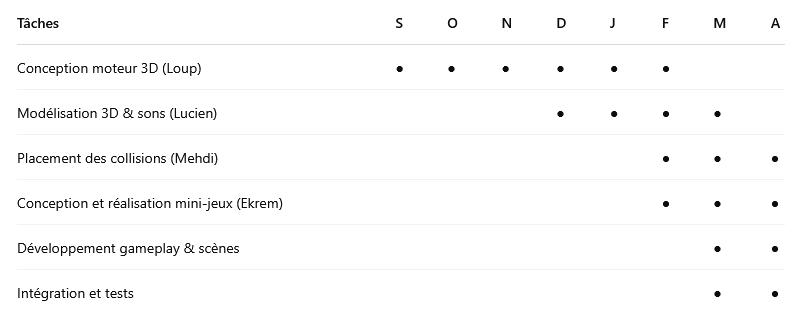
\includegraphics[width=0.6\textwidth]{images/gantt_effectif.png}
            \caption{Gantt effectif}
            \label{fig:gantt_effectif}
        \end{figure}
